\documentclass[letterpaper]{article}
\usepackage[margin=1in]{geometry}
\usepackage[utf8]{inputenc}
\usepackage{textcomp}
\usepackage{amssymb}
\usepackage{natbib}
\usepackage{graphicx}
\usepackage{gensymb}
\usepackage{amsthm, amsmath, mathtools}
\usepackage[dvipsnames]{xcolor}
\usepackage{enumerate}
\usepackage{mdframed}
\usepackage[most]{tcolorbox}
\usepackage{csquotes}
% https://tex.stackexchange.com/questions/13506/how-to-continue-the-framed-text-box-on-multiple-pages

\tcbuselibrary{theorems}

\newcommand{\R}{\mathbb{R}}
\newcommand{\Z}{\mathbb{Z}}
\newcommand{\N}{\mathbb{N}}
\newcommand{\Q}{\mathbb{Q}}
\newcommand{\C}{\mathbb{C}}
\newcommand{\code}[1]{\texttt{#1}}
\newcommand{\mdiamond}{$\diamondsuit$}
\newcommand{\PowerSet}{\mathcal{P}}
\newcommand{\Mod}[1]{\ (\mathrm{mod}\ #1)}
\DeclareMathOperator{\lcm}{lcm}

%\newtheorem*{theorem}{Theorem}
%\newtheorem*{definition}{Definition}
%\newtheorem*{corollary}{Corollary}
%\newtheorem*{lemma}{Lemma}
\newtheorem*{proposition}{Proposition}


\newtcbtheorem[number within=section]{theorem}{Theorem}
{colback=green!5,colframe=green!35!black,fonttitle=\bfseries}{th}

\newtcbtheorem[number within=section]{definition}{Definition}
{colback=blue!5,colframe=blue!35!black,fonttitle=\bfseries}{def}

\newtcbtheorem[number within=section]{corollary}{Corollary}
{colback=yellow!5,colframe=yellow!35!black,fonttitle=\bfseries}{cor}

\newtcbtheorem[number within=section]{lemma}{Lemma}
{colback=red!5,colframe=red!35!black,fonttitle=\bfseries}{lem}

\newtcbtheorem[number within=section]{example}{Example}
{colback=white!5,colframe=white!35!black,fonttitle=\bfseries}{def}

\newtcbtheorem[number within=section]{note}{Important Note}{
        enhanced,
        sharp corners,
        attach boxed title to top left={
            xshift=-1mm,
            yshift=-5mm,
            yshifttext=-1mm
        },
        top=1.5em,
        colback=white,
        colframe=black,
        fonttitle=\bfseries,
        boxed title style={
            sharp corners,
            size=small,
            colback=red!75!black,
            colframe=red!75!black,
        } 
    }{impnote}
\usepackage[utf8]{inputenc}
\usepackage[english]{babel}
\usepackage{fancyhdr}
\usepackage[hidelinks]{hyperref}

\pagestyle{fancy}
\fancyhf{}
\rhead{MATH 180A}
\chead{Friday, May 13, 2022}
\lhead{Lecture 20}
\rfoot{\thepage}

\setlength{\parindent}{0pt}

\begin{document}

\section{Central Limit Theorem}
Recall that the Law of Last Numbers says that if $X_1, X_2, \dots$ are IID with finite means $\mu$ and variances $\sigma^2$, then the averages $A_n = \frac{1}{n} \sum_{i = 1}^{n} X_i \mapsto \mu$. In particular, we proved the LLN using Chebychev's Inequality, which gives 
\[\PR\left(|A_n - \mu| \geq C \frac{\sigma}{\sqrt{n}}\right) \leq \frac{1}{C^2}.\] 

The \textbf{Central Limit Theorem (CLT)} says more. The Central Limit Theorem says that the normalized averages \[Z_n = \frac{A_n - \mu}{\sigma / \sqrt{n}}\] \emph{converge in distribution} (this sequence of RV converges to another RV) to a standard Normal(0, 1) random variable $Z$. More precisely, this means that the CDFs \[F_{Z_n}(z) \mapsto F_{Z}(z)\] as $n \mapsto \infty$. 

\begin{center}
    \begin{tabular}{||p{3in}|p{3in}||}
        \hline 
        \textbf{Chebyshev's Inequality} & \textbf{Central Limit Theorem} \\ 
        \hline \hline 
        \[\PR\left(|A_n - \mu| \geq C \frac{\sigma}{\sqrt{n}}\right) = \boxed{\PR(|Z_n| \geq C) \leq \frac{1}{C^2}}.\] 
        So, this gives us an upper-bound. Note that this works for \emph{any} $n$. 
        
        & 
        
        The CLT says that $\PR(|Z_n| \geq C) \mapsto \PR(|Z| \geq C)$, and 
        \[\PR(|Z| \geq C) = 2\int_{C}^{\infty} \frac{e^{-z^2 / 2}}{\sqrt{2\pi}} dz\]
        as $n \mapsto \infty$. Note that this works better for significantly large values of $n$.

        \bigskip 

        Note that \[\int_{C}^{\infty} \frac{e^{-z^2 / 2}}{\sqrt{2\pi}} dz\] is the area under the standard ``bell-shaped curve'' (i.e., the Normal(0, 1) PDF) to the right of $z = C$.
        \begin{center}
            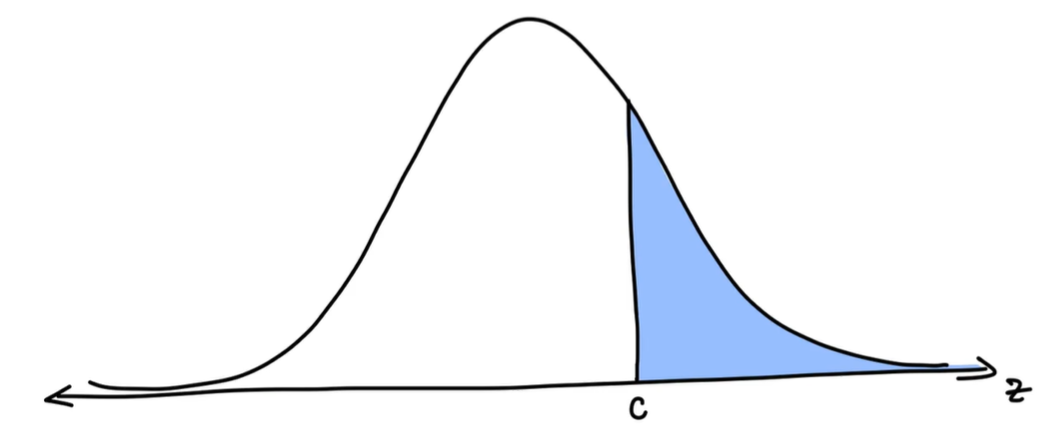
\includegraphics[scale=0.26]{../assets/lec20clt.png}
        \end{center}
        As a remark, the integral above doesn't have an antiderivative, but we can make use of an online $z$-score calculator to find (very good approximations to) these values.
        \\ 
        \hline 
    \end{tabular}
\end{center}
\textbf{Remark:} For this class, we usually let $\mu = 0$, $\sigma = 1$, and $x$ be the value of interest ($|Z|$, for example).

\begin{mdframed}[]
    (Example.) We note that, by using a $z$-score calculator, we know that 
    \[\PR(|Z| \geq 2) = 2\PR(Z \geq 2) \approx 4.55\%.\]
    Using Chebyshev's Inequality, we find that the upperbound is $\leq \frac{1}{2^2} = 25\%$. 
\end{mdframed}

\begin{theorem}{Central Limit Theorem}{}
    Suppose that $X_1, X_2, \dots$ are IID with common mean $\mu < \infty$ and variance $\sigma^2 < \infty$. Put \[S_n = \sum_{i = 1}^{n} X_i.\] Then, for any $b \in \R$, 
    \[\PR\left(\frac{S_n - n \mu}{\sigma\sqrt{n}} \leq b\right) \mapsto \frac{1}{\sqrt{2\pi}} \int_{-\infty}^{b} e^{-z^2 / 2}dz.\]
    Note that $\mathbb{E}(S_n) = n\mu$ and $SD(S_n) = \sqrt{\text{Var}(S_n)} = \sigma\sqrt{n}.$
\end{theorem}
\textbf{Remarks:} 
\begin{itemize}
    \item Note that 
    \[\frac{S_n - n\mu}{\sigma\sqrt{n}} = \frac{A_n - \mu}{\sigma / \sqrt{n}}\]
    where $S_n = \sum_{i = 1}^{n} X_i$ is the sum and $A_n = \frac{1}{n}S_n = \frac{1}{n} \sum_{i = 1}^{n} X_i$ is the average.  

    \item The key is that you do not need to know the actual distribution of the $X_i$'s. We only need to know that they are IIDs (and that their means are variances exist). So, in essense, \emph{the CLT gives useful information about averages of a distribution without needing to know what the distribution really is.}
\end{itemize}

Note that, when applying the CLT to \emph{discrete} IID sequences $X_1, X_2, \dots$, it is often useful to make a ``discrete adjustment'' to get a slightly better approximation. 

\begin{mdframed}[]
    (Example: Normal Approximation to the Binomial.) Recall that a Binomial($n, p$) RV $X_n$ is the sum of $n$ IID Bernoulli($p$) RVs, and that its mean is $np$ and variance $npq$, where $q = 1 - p$. Thus, by the CLT, 
    \[\PR(i \leq X_n \leq j) \approx \PR\left(\frac{i - np}{\sqrt{npq}} \leq Z \leq \frac{j - np}{\sqrt{npq}}\right)\]
    for large $n$.

    \bigskip 

    We can, however, get a better approximation (unless $n$ is very large, in which case it makes little difference) if we instead approximate
    \[\PR(i \leq X_n \leq j) \approx \PR\left(\frac{i - 1/2 - np}{\sqrt{npq}} \leq Z \leq \frac{j + 1/2 - np}{\sqrt{npq}}\right).\]
    The reason why is because this makes a correction to get all of the relevant ``bars.''
\end{mdframed}

\begin{mdframed}[]
    (Example.) A fair coin is tossed 100 times. Estimate the probability that ``Heads'' is tossed between 40 and 60 times. 

    \bigskip 

    Let $S_n = \sum_{i = 1}^{n} X_i$ where $X_i$ indicates if the $i$th toss is ``Heads.'' Letting $X_i$ be a Bernoulli, where $X_i$ is 1 if the $i$th toss is ``Heads'' and 0 otherwise. Then, applying the Binomial approximation, we have  
    \begin{equation*}
        \begin{aligned}
            \PR(40 \leq S_n \leq 60) &= \PR\left(\frac{40 - 0.5 - 100(0.5)}{\sqrt{100(0.5)(1 - 0.5)}} \leq Z \leq \frac{60 + 0.5 - 100(0.5)}{\sqrt{100(0.5)(1 - 0.5)}}\right) \\ 
                &= \PR(|Z| \leq 2.1).
        \end{aligned}
    \end{equation*}
    So, using the online calculator, we want to compute 
    \[\PR(-2.1 \leq Z \leq 2.1).\]
    Doing this (letting $\mu = 0$, $\sigma = 1$, $x = 2.1$, and $\PR(-|x| < X < |x|)$ in the dropdown menu) gives us 96.42\%.

    \bigskip 

    Without the discrete correction, we would have found 
    \[\PR(-2 \leq Z \leq 2) \approx 95.45\%.\]
    But, by calculating the true probability, we get 
    \[\frac{1}{2^{100}} \sum_{i = 40}^{60} \binom{100}{i} = 96.479\dots\%.\]
\end{mdframed}


\begin{theorem}{}{}
    If the $X_1, X_2, \dots$ are independent with means $\mu_i < \infty$ and variances $\sigma^2 < \infty$, and such that for some constant $A < \infty$, all $|X_i| \leq A$ (i.e., the $X_i$ are ``uniformly bounded''), then the conclusion of the CLT still holds; that is, 
    \[\PR\left(\frac{S_n - \mathbb{E}(S_n)}{SD(S_n) \leq b}\right) \mapsto \frac{1}{\sqrt{2\pi}} \int_{-\infty}^{b} e^{-z^2 / 2}dz.\]
\end{theorem}
\textbf{Remark:} Note that $\mathbb{E}(S_n) = \sum_{i = 1}^{n} \mu_i$ and $SD(S_n) = \sqrt{\sum_{i = 1}^{n} \sigma_i^2}$. 

\textbf{Course Note:} This will not be tested on homework assignments or exams.

\end{document}